% Indicate the main file. Must go at the beginning of the file.
% !TEX root = ../main.tex

%----------------------------------------------------------------------------------------
% CHAPTER 2
%----------------------------------------------------------------------------------------

\chapter{Theory}

\label{Chapter2} % For referencing the chapter elsewhere, use \ref{Chapter2} 

%----------------------------------------------------------------------------------------


\section{X-ray photoelectron spectroscopic analysis}

\subsection{Principle of measurement}


In X-ray photoelectron spectroscopy, soft x-rays are most commonly generated by exciting Al or Mg to radiate K \(\alpha\) x-rays with 1486.6 eV and 1253.6 eV respectively. These x-ray sources have a small natural linewidth and thus can provide high resolution. The photons then interact with the sample which in turn emit electrons due to the photoelectric effect. Those electrons are then transported to a multichannel detector which counts the electrons. To improve, detector efficiency and electron collection, and thus the resolution, a monochromator is usually used.\cite{stevie_introduction_2020} The concept of the measurement can be expressed as shown in eq. 1:
\begin{equation}
    hv = BE + KE + \psi spec
\end{equation}
which can be re-arranged to express the binding energy as a function of known variables \cite{stevie_introduction_2020} as shown in eq. 2
\begin{equation}
    BE = hv- KE - \psi spec
\end{equation}

The complex and sample-specific interactions of the produced electrons with the sample are discussed in the next chapter.
 
The sample work function is a specific change in energy levels dependent on the chemical environment (coordination, charge etc.) of the atom of interest. It describes the work an electron must overcome to escape the local environment up to the vacuum level.

The intensity of the peaks is indicated as counts and corresponds to the number of electrons that reach the detector during the acquisition time. Thus, the intensity of the signal depends on the acquisition time and should be normalized before comparing with spectra collected with unknown method and instrument parameters. 



\subsection{Surface sensitivity}

The study of surface sensitivity in XPS has been thoroughly studied and summarized in multiple publications \cite{powell_surface_2009, }. Electrons emitted from the samples atoms can take different ways until they reach the detector. They either take a direct path which is the predominant proportion at the most outer 


To this point, there are three terms to describe surface sensitivity in XPS.
\begin{itemize}
\item The initial energy which is needed to overcome dielectric effects such that an electron can be lost from a material is described by the electron loss function (ELF)
\item Inelastic mean free path (IMFP) describes the distance an electron travels in a given material before inelastically scattering.
\item Electron attenuation length (EAL) is the length the electron travels into the sample.

\end{itemize}

Elastic electron scattering, however, has often caused uncertainties in measurements of EAL and IMFP. 
The IMFP is element specific and also depends on the kinetic energy 
\begin{figure}
    \centering
    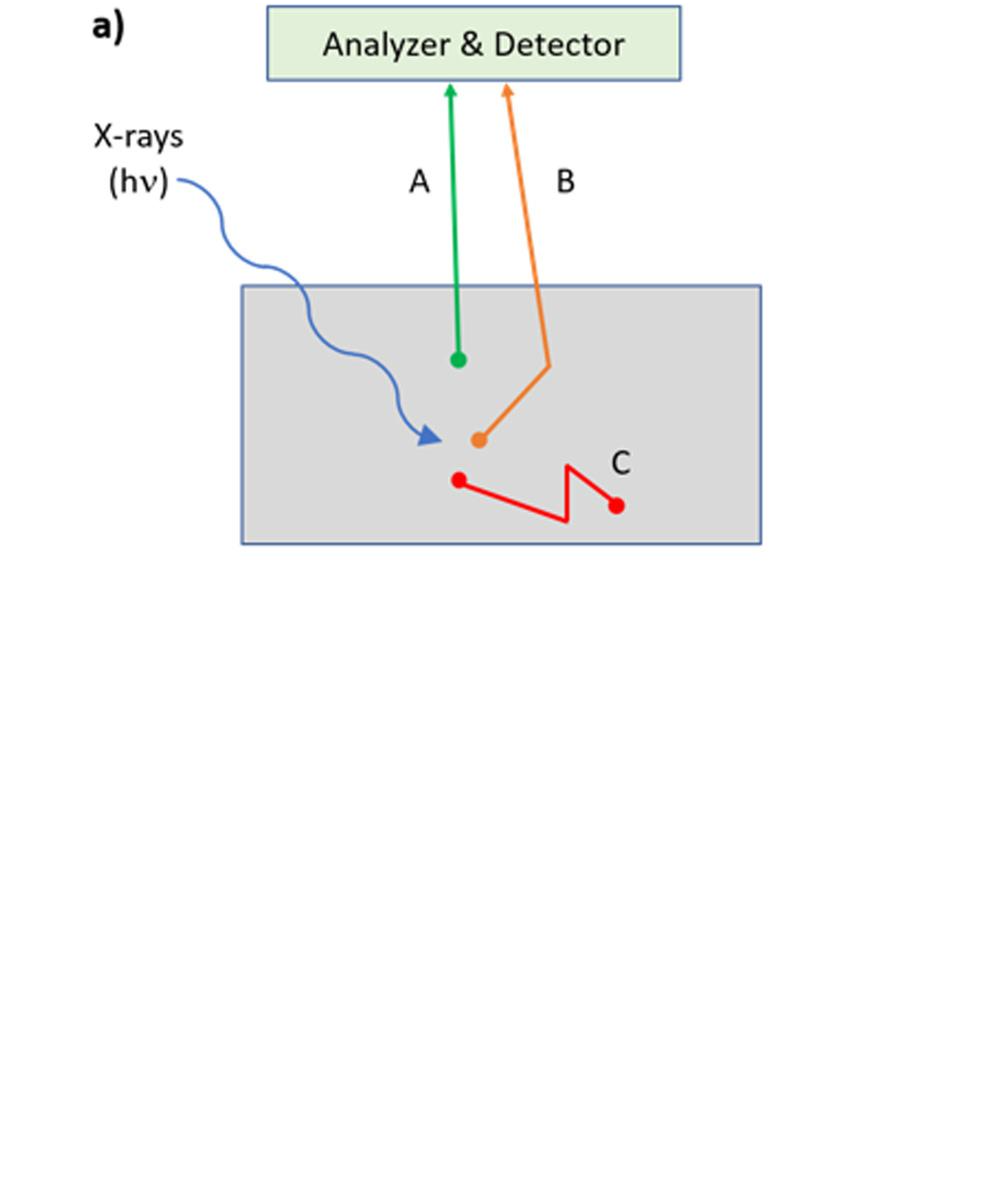
\includegraphics[scale=0.3]{Figures/image6_1.png}
    \caption{Scattering effects in XPS \cite{stevie_introduction_2020}}
    \label{fig:scattering}
\end{figure}

\subsection{Depth profiling}

Experimentally, there exist four methods for investigating depth-information of a component in a sample. These are:
\begin{enumerate}
    \item presence or absence of energy loss peaks
    \item the intensity ratio of peaks across the kinetic energy (high vs low) – only suitable for a selection of elements (semi-qualitative).
    \item controlled erosion and subsequent measurement of the surface (destructive and high material dependency)
    \item measurement at different sample-mounting angles (ARXPS). \cite{moulder_handbook_1992} 

and more recently have been extended by two additional methods:

    \item Combination with hard x-ray photoelectron spectroscopy (HAXPES) has become more accessible which in combination with XPS can give depth information of a sample \cite{zborowski_improved_2022}.
    \item Modelling of X-ray photoelectron spectra another recent technique for the determination of depth distribution and has been investigated previously using manual approaches \cite{zborowski_comparison_2022}.

\end{enumerate}


The methods 1-3 have the drawback of being potentially destructive on the sample surface. Further, they are giving only very vague information about the samples’ depth profile; the accuracy is often denoted to be $\pm$10\%.

The non-destructive methods 4-6 (ARXPS / Modelling / XPS-HAXPES) are further explained, as they are comparable to our data-driven approach. 

\subsection{Deep learning for spectroscopic data}
Techniques of machine learning and deep learning specifically have been applied to spectroscopic data for a long time. However, chemometric or physics-based approaches have been and still are favored for data analysis due to the lack of model explainability for data-driven approaches.





%----------------------------------------------------------------------------------------

%\lstinputlisting[language=Python,caption=External file: code/example.py]{Code/example.py}
